\clearpage
\section{Оценка качества синтеза текстур с трендом}
	После обучения сети, необходимо проверить, что сгенерированные ей изображения действительно имеют искомые характеристики (то есть, содержат искомый тренд). Для этого вводится специальная метрика, которая будет учитывать наличие в изображении тренда интенсивности частиц. Рассмотрим среднюю плотность черных пикселей в некотором окне $\xi_k$, и пройдем этим окном по изображению.
	$$\xi_k = \frac{1}{H w}{\sum_{i=k}^{k+w} \sum_{j=0}^{H}\left| \frac{x(i, j) - 255}{255} \right|}, $$$$k = \overline{1, W - w} $$
	
	Построив график $\xi(k)$, можно увидеть, как меняется плотность черных пикселей и прослеживается ли тренд (Рис. \ref{7-window}).
	
	\begin{figure}[h!]
		\centering{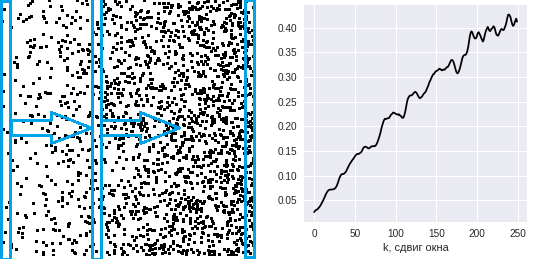
\includegraphics[width=0.75\linewidth]{7-verification/window}}
		\caption{Прохождение окном, W, H - размеры изображения, w - ширина окна.}
		\label{7-window}
	\end{figure}
	
	В качестве метрики можно взять среднеквадратичную ошибку:
	$$ \xi = \frac{K}{W-w}\sum_{k=1}^{W-w} (\xi_k - \xi_{0k})^2,$$
	где $\xi_{0k}$ - это $\xi_k$, усредненное по изображениям, содержащим истинный тренд, а $K$ - нормировочный множитель, вводимый для того, чтобы метрики сетей, обученных на разных выборках можно было сравнивать между собой. Соответственно, чем меньше значение метрики, тем лучше тренд, присутствующий на сгенерированном изображении, приближает искомый.